\documentclass[aps,10pt,prd,twocolumn,floats,letterpaper,showpacs,nofootinbib,bibnotes,notitlepage,superscriptaddress,floatfix]{revtex4-1}

\usepackage{graphicx}
\usepackage{mathrsfs}
\usepackage[intlimits,centertags]{amsmath}
\usepackage{amssymb,amsfonts}
\usepackage[pdftex]{hyperref}
\usepackage[x11names]{xcolor}
\usepackage{enumerate}
\usepackage{xfrac}
\usepackage[normalem]{ulem}
\usepackage{float}

\usepackage{lineno}
\linenumbers

\newcommand{\MA}[1]{{\color{magenta}#1}}

\begin{document}

\title{IceCube Data for Neutrino Point-Source Searches: Years 2012--2018}

\author{\MA{IceCube author list in final version}}
%\affiliation{III. Physikalisches Institut, RWTH Aachen University, D-52056 Aachen, Germany}
\affiliation{Department of Physics, University of Adelaide, Adelaide, 5005, Australia}
\affiliation{Dept. of Physics and Astronomy, University of Alaska Anchorage, 3211 Providence Dr., Anchorage, AK 99508, USA}
\affiliation{Dept. of Physics, University of Texas at Arlington, 502 Yates St., Science Hall Rm 108, Box 19059, Arlington, TX 76019, USA}
\affiliation{CTSPS, Clark-Atlanta University, Atlanta, GA 30314, USA}
\affiliation{School of Physics and Center for Relativistic Astrophysics, Georgia Institute of Technology, Atlanta, GA 30332, USA}
\affiliation{Dept. of Physics, Southern University, Baton Rouge, LA 70813, USA}
\affiliation{Dept. of Physics, University of California, Berkeley, CA 94720, USA}
\affiliation{Lawrence Berkeley National Laboratory, Berkeley, CA 94720, USA}
\affiliation{Institut f{\"u}r Physik, Humboldt-Universit{\"a}t zu Berlin, D-12489 Berlin, Germany}
\affiliation{Fakult{\"a}t f{\"u}r Physik {\&} Astronomie, Ruhr-Universit{\"a}t Bochum, D-44780 Bochum, Germany}
\affiliation{Universit{\'e} Libre de Bruxelles, Science Faculty CP230, B-1050 Brussels, Belgium}
\affiliation{Vrije Universiteit Brussel (VUB), Dienst ELEM, B-1050 Brussels, Belgium}
\affiliation{Department of Physics and Laboratory for Particle Physics and Cosmology, Harvard University, Cambridge, MA 02138, USA}
\affiliation{Dept. of Physics, Massachusetts Institute of Technology, Cambridge, MA 02139, USA}
\affiliation{Dept. of Physics and Institute for Global Prominent Research, Chiba University, Chiba 263-8522, Japan}
\affiliation{Department of Physics, Loyola University Chicago, Chicago, IL 60660, USA}
\affiliation{Dept. of Physics and Astronomy, University of Canterbury, Private Bag 4800, Christchurch, New Zealand}
\affiliation{Dept. of Physics, University of Maryland, College Park, MD 20742, USA}
\affiliation{Dept. of Astronomy, Ohio State University, Columbus, OH 43210, USA}
\affiliation{Dept. of Physics and Center for Cosmology and Astro-Particle Physics, Ohio State University, Columbus, OH 43210, USA}
\affiliation{Niels Bohr Institute, University of Copenhagen, DK-2100 Copenhagen, Denmark}
\affiliation{Dept. of Physics, TU Dortmund University, D-44221 Dortmund, Germany}
\affiliation{Dept. of Physics and Astronomy, Michigan State University, East Lansing, MI 48824, USA}
\affiliation{Dept. of Physics, University of Alberta, Edmonton, Alberta, Canada T6G 2E1}
\affiliation{Erlangen Centre for Astroparticle Physics, Friedrich-Alexander-Universit{\"a}t Erlangen-N{\"u}rnberg, D-91058 Erlangen, Germany}
\affiliation{Physik-department, Technische Universit{\"a}t M{\"u}nchen, D-85748 Garching, Germany}
\affiliation{D{\'e}partement de physique nucl{\'e}aire et corpusculaire, Universit{\'e} de Gen{\`e}ve, CH-1211 Gen{\`e}ve, Switzerland}
\affiliation{Dept. of Physics and Astronomy, University of Gent, B-9000 Gent, Belgium}
\affiliation{Dept. of Physics and Astronomy, University of California, Irvine, CA 92697, USA}
\affiliation{Karlsruhe Institute of Technology, Institut f{\"u}r Kernphysik, D-76021 Karlsruhe, Germany}
\affiliation{Dept. of Physics and Astronomy, University of Kansas, Lawrence, KS 66045, USA}
\affiliation{SNOLAB, 1039 Regional Road 24, Creighton Mine 9, Lively, ON, Canada P3Y 1N2}
\affiliation{Department of Physics and Astronomy, UCLA, Los Angeles, CA 90095, USA}
\affiliation{Department of Physics, Mercer University, Macon, GA 31207-0001, USA}
\affiliation{Dept. of Astronomy, University of Wisconsin{\textendash}Madison, Madison, WI 53706, USA}
\affiliation{Dept. of Physics and Wisconsin IceCube Particle Astrophysics Center, University of Wisconsin{\textendash}Madison, Madison, WI 53706, USA}
\affiliation{Institute of Physics, University of Mainz, Staudinger Weg 7, D-55099 Mainz, Germany}
\affiliation{Department of Physics, Marquette University, Milwaukee, WI, 53201, USA}
\affiliation{Institut f{\"u}r Kernphysik, Westf{\"a}lische Wilhelms-Universit{\"a}t M{\"u}nster, D-48149 M{\"u}nster, Germany}
\affiliation{Bartol Research Institute and Dept. of Physics and Astronomy, University of Delaware, Newark, DE 19716, USA}
\affiliation{Dept. of Physics, Yale University, New Haven, CT 06520, USA}
\affiliation{Dept. of Physics, University of Oxford, Parks Road, Oxford OX1 3PU, UK}
\affiliation{Dept. of Physics, Drexel University, 3141 Chestnut Street, Philadelphia, PA 19104, USA}
\affiliation{Physics Department, South Dakota School of Mines and Technology, Rapid City, SD 57701, USA}
\affiliation{Dept. of Physics, University of Wisconsin, River Falls, WI 54022, USA}
\affiliation{Dept. of Physics and Astronomy, University of Rochester, Rochester, NY 14627, USA}
\affiliation{Oskar Klein Centre and Dept. of Physics, Stockholm University, SE-10691 Stockholm, Sweden}
\affiliation{Dept. of Physics and Astronomy, Stony Brook University, Stony Brook, NY 11794-3800, USA}
\affiliation{Dept. of Physics, Sungkyunkwan University, Suwon 16419, Korea}
\affiliation{Institute of Basic Science, Sungkyunkwan University, Suwon 16419, Korea}
\affiliation{Dept. of Physics and Astronomy, University of Alabama, Tuscaloosa, AL 35487, USA}
\affiliation{Dept. of Astronomy and Astrophysics, Pennsylvania State University, University Park, PA 16802, USA}
\affiliation{Dept. of Physics, Pennsylvania State University, University Park, PA 16802, USA}
\affiliation{Dept. of Physics and Astronomy, Uppsala University, Box 516, S-75120 Uppsala, Sweden}
\affiliation{Dept. of Physics, University of Wuppertal, D-42119 Wuppertal, Germany}
\affiliation{DESY, D-15738 Zeuthen, Germany}

\author{R. Abbasi}
\affiliation{Department of Physics, Loyola University Chicago, Chicago, IL 60660, USA}
\author{M. Ackermann}
\affiliation{DESY, D-15738 Zeuthen, Germany}
\author{J. Adams}
\affiliation{Dept. of Physics and Astronomy, University of Canterbury, Private Bag 4800, Christchurch, New Zealand}
\author{J. A. Aguilar}
\affiliation{Universit{\'e} Libre de Bruxelles, Science Faculty CP230, B-1050 Brussels, Belgium}
\author{M. Ahlers}
\affiliation{Niels Bohr Institute, University of Copenhagen, DK-2100 Copenhagen, Denmark}
\author{M. Ahrens}
\affiliation{Oskar Klein Centre and Dept. of Physics, Stockholm University, SE-10691 Stockholm, Sweden}
\author{C. Alispach}
\affiliation{D{\'e}partement de physique nucl{\'e}aire et corpusculaire, Universit{\'e} de Gen{\`e}ve, CH-1211 Gen{\`e}ve, Switzerland}
\author{N. M. Amin}
\affiliation{Bartol Research Institute and Dept. of Physics and Astronomy, University of Delaware, Newark, DE 19716, USA}
\author{K. Andeen}
\affiliation{Department of Physics, Marquette University, Milwaukee, WI, 53201, USA}
\author{T. Anderson}
\affiliation{Dept. of Physics, Pennsylvania State University, University Park, PA 16802, USA}
\author{I. Ansseau}
\affiliation{Universit{\'e} Libre de Bruxelles, Science Faculty CP230, B-1050 Brussels, Belgium}
\author{G. Anton}
\affiliation{Erlangen Centre for Astroparticle Physics, Friedrich-Alexander-Universit{\"a}t Erlangen-N{\"u}rnberg, D-91058 Erlangen, Germany}
\author{C. Arg{\"u}elles}
\affiliation{Department of Physics and Laboratory for Particle Physics and Cosmology, Harvard University, Cambridge, MA 02138, USA}
\author{S. Axani}
\affiliation{Dept. of Physics, Massachusetts Institute of Technology, Cambridge, MA 02139, USA}
\author{X. Bai}
\affiliation{Physics Department, South Dakota School of Mines and Technology, Rapid City, SD 57701, USA}
\author{A. Balagopal V.}
\affiliation{Karlsruhe Institute of Technology, Institut f{\"u}r Kernphysik, D-76021 Karlsruhe, Germany}
\author{A. Barbano}
\affiliation{D{\'e}partement de physique nucl{\'e}aire et corpusculaire, Universit{\'e} de Gen{\`e}ve, CH-1211 Gen{\`e}ve, Switzerland}
\author{S. W. Barwick}
\affiliation{Dept. of Physics and Astronomy, University of California, Irvine, CA 92697, USA}
\author{B. Bastian}
\affiliation{DESY, D-15738 Zeuthen, Germany}
\author{V. Basu}
\affiliation{Dept. of Physics and Wisconsin IceCube Particle Astrophysics Center, University of Wisconsin{\textendash}Madison, Madison, WI 53706, USA}
\author{V. Baum}
\affiliation{Institute of Physics, University of Mainz, Staudinger Weg 7, D-55099 Mainz, Germany}
\author{S. Baur}
\affiliation{Universit{\'e} Libre de Bruxelles, Science Faculty CP230, B-1050 Brussels, Belgium}
\author{R. Bay}
\affiliation{Dept. of Physics, University of California, Berkeley, CA 94720, USA}
\author{J. J. Beatty}
\affiliation{Dept. of Astronomy, Ohio State University, Columbus, OH 43210, USA}
\affiliation{Dept. of Physics and Center for Cosmology and Astro-Particle Physics, Ohio State University, Columbus, OH 43210, USA}
\author{K.-H. Becker}
\affiliation{Dept. of Physics, University of Wuppertal, D-42119 Wuppertal, Germany}
\author{J. Becker Tjus}
\affiliation{Fakult{\"a}t f{\"u}r Physik {\&} Astronomie, Ruhr-Universit{\"a}t Bochum, D-44780 Bochum, Germany}
\author{C. Bellenghi}
\affiliation{Physik-department, Technische Universit{\"a}t M{\"u}nchen, D-85748 Garching, Germany}
\author{S. BenZvi}
\affiliation{Dept. of Physics and Astronomy, University of Rochester, Rochester, NY 14627, USA}
\author{D. Berley}
\affiliation{Dept. of Physics, University of Maryland, College Park, MD 20742, USA}
\author{E. Bernardini}
\thanks{also at Universit{\`a} di Padova, I-35131 Padova, Italy}
\affiliation{DESY, D-15738 Zeuthen, Germany}
\author{D. Z. Besson}
\thanks{also at National Research Nuclear University, Moscow Engineering Physics Institute (MEPhI), Moscow 115409, Russia}
\affiliation{Dept. of Physics and Astronomy, University of Kansas, Lawrence, KS 66045, USA}
\author{G. Binder}
\affiliation{Dept. of Physics, University of California, Berkeley, CA 94720, USA}
\affiliation{Lawrence Berkeley National Laboratory, Berkeley, CA 94720, USA}
\author{D. Bindig}
\affiliation{Dept. of Physics, University of Wuppertal, D-42119 Wuppertal, Germany}
\author{E. Blaufuss}
\affiliation{Dept. of Physics, University of Maryland, College Park, MD 20742, USA}
\author{S. Blot}
\affiliation{DESY, D-15738 Zeuthen, Germany}
\author{C. Bohm}
\affiliation{Oskar Klein Centre and Dept. of Physics, Stockholm University, SE-10691 Stockholm, Sweden}
\author{S. B{\"o}ser}
\affiliation{Institute of Physics, University of Mainz, Staudinger Weg 7, D-55099 Mainz, Germany}
\author{O. Botner}
\affiliation{Dept. of Physics and Astronomy, Uppsala University, Box 516, S-75120 Uppsala, Sweden}
\author{J. B{\"o}ttcher}
\affiliation{III. Physikalisches Institut, RWTH Aachen University, D-52056 Aachen, Germany}
\author{E. Bourbeau}
\affiliation{Niels Bohr Institute, University of Copenhagen, DK-2100 Copenhagen, Denmark}
\author{J. Bourbeau}
\affiliation{Dept. of Physics and Wisconsin IceCube Particle Astrophysics Center, University of Wisconsin{\textendash}Madison, Madison, WI 53706, USA}
\author{F. Bradascio}
\affiliation{DESY, D-15738 Zeuthen, Germany}
\author{J. Braun}
\affiliation{Dept. of Physics and Wisconsin IceCube Particle Astrophysics Center, University of Wisconsin{\textendash}Madison, Madison, WI 53706, USA}
\author{S. Bron}
\affiliation{D{\'e}partement de physique nucl{\'e}aire et corpusculaire, Universit{\'e} de Gen{\`e}ve, CH-1211 Gen{\`e}ve, Switzerland}
\author{J. Brostean-Kaiser}
\affiliation{DESY, D-15738 Zeuthen, Germany}
\author{A. Burgman}
\affiliation{Dept. of Physics and Astronomy, Uppsala University, Box 516, S-75120 Uppsala, Sweden}
\author{J. Buscher}
\affiliation{III. Physikalisches Institut, RWTH Aachen University, D-52056 Aachen, Germany}
\author{R. S. Busse}
\affiliation{Institut f{\"u}r Kernphysik, Westf{\"a}lische Wilhelms-Universit{\"a}t M{\"u}nster, D-48149 M{\"u}nster, Germany}
\author{M. A. Campana}
\affiliation{Dept. of Physics, Drexel University, 3141 Chestnut Street, Philadelphia, PA 19104, USA}
\author{T. Carver}
\affiliation{D{\'e}partement de physique nucl{\'e}aire et corpusculaire, Universit{\'e} de Gen{\`e}ve, CH-1211 Gen{\`e}ve, Switzerland}
\author{C. Chen}
\affiliation{School of Physics and Center for Relativistic Astrophysics, Georgia Institute of Technology, Atlanta, GA 30332, USA}
\author{E. Cheung}
\affiliation{Dept. of Physics, University of Maryland, College Park, MD 20742, USA}
\author{D. Chirkin}
\affiliation{Dept. of Physics and Wisconsin IceCube Particle Astrophysics Center, University of Wisconsin{\textendash}Madison, Madison, WI 53706, USA}
\author{S. Choi}
\affiliation{Dept. of Physics, Sungkyunkwan University, Suwon 16419, Korea}
\author{B. A. Clark}
\affiliation{Dept. of Physics and Astronomy, Michigan State University, East Lansing, MI 48824, USA}
\author{K. Clark}
\affiliation{SNOLAB, 1039 Regional Road 24, Creighton Mine 9, Lively, ON, Canada P3Y 1N2}
\author{L. Classen}
\affiliation{Institut f{\"u}r Kernphysik, Westf{\"a}lische Wilhelms-Universit{\"a}t M{\"u}nster, D-48149 M{\"u}nster, Germany}
\author{A. Coleman}
\affiliation{Bartol Research Institute and Dept. of Physics and Astronomy, University of Delaware, Newark, DE 19716, USA}
\author{G. H. Collin}
\affiliation{Dept. of Physics, Massachusetts Institute of Technology, Cambridge, MA 02139, USA}
\author{J. M. Conrad}
\affiliation{Dept. of Physics, Massachusetts Institute of Technology, Cambridge, MA 02139, USA}
\author{P. Coppin}
\affiliation{Vrije Universiteit Brussel (VUB), Dienst ELEM, B-1050 Brussels, Belgium}
\author{P. Correa}
\affiliation{Vrije Universiteit Brussel (VUB), Dienst ELEM, B-1050 Brussels, Belgium}
\author{D. F. Cowen}
\affiliation{Dept. of Astronomy and Astrophysics, Pennsylvania State University, University Park, PA 16802, USA}
\affiliation{Dept. of Physics, Pennsylvania State University, University Park, PA 16802, USA}
\author{R. Cross}
\affiliation{Dept. of Physics and Astronomy, University of Rochester, Rochester, NY 14627, USA}
\author{P. Dave}
\affiliation{School of Physics and Center for Relativistic Astrophysics, Georgia Institute of Technology, Atlanta, GA 30332, USA}
\author{C. De Clercq}
\affiliation{Vrije Universiteit Brussel (VUB), Dienst ELEM, B-1050 Brussels, Belgium}
\author{J. J. DeLaunay}
\affiliation{Dept. of Physics, Pennsylvania State University, University Park, PA 16802, USA}
\author{H. Dembinski}
\affiliation{Bartol Research Institute and Dept. of Physics and Astronomy, University of Delaware, Newark, DE 19716, USA}
\author{K. Deoskar}
\affiliation{Oskar Klein Centre and Dept. of Physics, Stockholm University, SE-10691 Stockholm, Sweden}
\author{S. De Ridder}
\affiliation{Dept. of Physics and Astronomy, University of Gent, B-9000 Gent, Belgium}
\author{A. Desai}
\affiliation{Dept. of Physics and Wisconsin IceCube Particle Astrophysics Center, University of Wisconsin{\textendash}Madison, Madison, WI 53706, USA}
\author{P. Desiati}
\affiliation{Dept. of Physics and Wisconsin IceCube Particle Astrophysics Center, University of Wisconsin{\textendash}Madison, Madison, WI 53706, USA}
\author{K. D. de Vries}
\affiliation{Vrije Universiteit Brussel (VUB), Dienst ELEM, B-1050 Brussels, Belgium}
\author{G. de Wasseige}
\affiliation{Vrije Universiteit Brussel (VUB), Dienst ELEM, B-1050 Brussels, Belgium}
\author{M. de With}
\affiliation{Institut f{\"u}r Physik, Humboldt-Universit{\"a}t zu Berlin, D-12489 Berlin, Germany}
\author{T. DeYoung}
\affiliation{Dept. of Physics and Astronomy, Michigan State University, East Lansing, MI 48824, USA}
\author{S. Dharani}
\affiliation{III. Physikalisches Institut, RWTH Aachen University, D-52056 Aachen, Germany}
\author{A. Diaz}
\affiliation{Dept. of Physics, Massachusetts Institute of Technology, Cambridge, MA 02139, USA}
\author{J. C. D{\'\i}az-V{\'e}lez}
\affiliation{Dept. of Physics and Wisconsin IceCube Particle Astrophysics Center, University of Wisconsin{\textendash}Madison, Madison, WI 53706, USA}
\author{H. Dujmovic}
\affiliation{Karlsruhe Institute of Technology, Institut f{\"u}r Kernphysik, D-76021 Karlsruhe, Germany}
\author{M. Dunkman}
\affiliation{Dept. of Physics, Pennsylvania State University, University Park, PA 16802, USA}
\author{M. A. DuVernois}
\affiliation{Dept. of Physics and Wisconsin IceCube Particle Astrophysics Center, University of Wisconsin{\textendash}Madison, Madison, WI 53706, USA}
\author{E. Dvorak}
\affiliation{Physics Department, South Dakota School of Mines and Technology, Rapid City, SD 57701, USA}
\author{T. Ehrhardt}
\affiliation{Institute of Physics, University of Mainz, Staudinger Weg 7, D-55099 Mainz, Germany}
\author{P. Eller}
\affiliation{Physik-department, Technische Universit{\"a}t M{\"u}nchen, D-85748 Garching, Germany}
\author{R. Engel}
\affiliation{Karlsruhe Institute of Technology, Institut f{\"u}r Kernphysik, D-76021 Karlsruhe, Germany}
\author{P. A. Evenson}
\affiliation{Bartol Research Institute and Dept. of Physics and Astronomy, University of Delaware, Newark, DE 19716, USA}
\author{S. Fahey}
\affiliation{Dept. of Physics and Wisconsin IceCube Particle Astrophysics Center, University of Wisconsin{\textendash}Madison, Madison, WI 53706, USA}
\author{A. R. Fazely}
\affiliation{Dept. of Physics, Southern University, Baton Rouge, LA 70813, USA}
\author{J. Felde}
\affiliation{Dept. of Physics, University of Maryland, College Park, MD 20742, USA}
\author{A.T. Fienberg}
\affiliation{Dept. of Physics, Pennsylvania State University, University Park, PA 16802, USA}
\author{K. Filimonov}
\affiliation{Dept. of Physics, University of California, Berkeley, CA 94720, USA}
\author{C. Finley}
\affiliation{Oskar Klein Centre and Dept. of Physics, Stockholm University, SE-10691 Stockholm, Sweden}
\author{L. Fischer}
\affiliation{DESY, D-15738 Zeuthen, Germany}
\author{D. Fox}
\affiliation{Dept. of Astronomy and Astrophysics, Pennsylvania State University, University Park, PA 16802, USA}
\author{A. Franckowiak}
\affiliation{DESY, D-15738 Zeuthen, Germany}
\author{E. Friedman}
\affiliation{Dept. of Physics, University of Maryland, College Park, MD 20742, USA}
\author{A. Fritz}
\affiliation{Institute of Physics, University of Mainz, Staudinger Weg 7, D-55099 Mainz, Germany}
\author{T. K. Gaisser}
\affiliation{Bartol Research Institute and Dept. of Physics and Astronomy, University of Delaware, Newark, DE 19716, USA}
\author{J. Gallagher}
\affiliation{Dept. of Astronomy, University of Wisconsin{\textendash}Madison, Madison, WI 53706, USA}
\author{E. Ganster}
\affiliation{III. Physikalisches Institut, RWTH Aachen University, D-52056 Aachen, Germany}
\author{S. Garrappa}
\affiliation{DESY, D-15738 Zeuthen, Germany}
\author{L. Gerhardt}
\affiliation{Lawrence Berkeley National Laboratory, Berkeley, CA 94720, USA}
\author{A. Ghadimi}
\affiliation{Dept. of Physics and Astronomy, University of Alabama, Tuscaloosa, AL 35487, USA}
\author{T. Glauch}
\affiliation{Physik-department, Technische Universit{\"a}t M{\"u}nchen, D-85748 Garching, Germany}
\author{T. Gl{\"u}senkamp}
\affiliation{Erlangen Centre for Astroparticle Physics, Friedrich-Alexander-Universit{\"a}t Erlangen-N{\"u}rnberg, D-91058 Erlangen, Germany}
\author{A. Goldschmidt}
\affiliation{Lawrence Berkeley National Laboratory, Berkeley, CA 94720, USA}
\author{J. G. Gonzalez}
\affiliation{Bartol Research Institute and Dept. of Physics and Astronomy, University of Delaware, Newark, DE 19716, USA}
\author{S. Goswami}
\affiliation{Dept. of Physics and Astronomy, University of Alabama, Tuscaloosa, AL 35487, USA}
\author{D. Grant}
\affiliation{Dept. of Physics and Astronomy, Michigan State University, East Lansing, MI 48824, USA}
\author{T. Gr{\'e}goire}
\affiliation{Dept. of Physics, Pennsylvania State University, University Park, PA 16802, USA}
\author{Z. Griffith}
\affiliation{Dept. of Physics and Wisconsin IceCube Particle Astrophysics Center, University of Wisconsin{\textendash}Madison, Madison, WI 53706, USA}
\author{S. Griswold}
\affiliation{Dept. of Physics and Astronomy, University of Rochester, Rochester, NY 14627, USA}
\author{M. G{\"u}nd{\"u}z}
\affiliation{Fakult{\"a}t f{\"u}r Physik {\&} Astronomie, Ruhr-Universit{\"a}t Bochum, D-44780 Bochum, Germany}
\author{C. Haack}
\affiliation{Physik-department, Technische Universit{\"a}t M{\"u}nchen, D-85748 Garching, Germany}
\author{A. Hallgren}
\affiliation{Dept. of Physics and Astronomy, Uppsala University, Box 516, S-75120 Uppsala, Sweden}
\author{R. Halliday}
\affiliation{Dept. of Physics and Astronomy, Michigan State University, East Lansing, MI 48824, USA}
\author{L. Halve}
\affiliation{III. Physikalisches Institut, RWTH Aachen University, D-52056 Aachen, Germany}
\author{F. Halzen}
\affiliation{Dept. of Physics and Wisconsin IceCube Particle Astrophysics Center, University of Wisconsin{\textendash}Madison, Madison, WI 53706, USA}
\author{M. Ha Minh}
\affiliation{Physik-department, Technische Universit{\"a}t M{\"u}nchen, D-85748 Garching, Germany}
\author{K. Hanson}
\affiliation{Dept. of Physics and Wisconsin IceCube Particle Astrophysics Center, University of Wisconsin{\textendash}Madison, Madison, WI 53706, USA}
\author{J. Hardin}
\affiliation{Dept. of Physics and Wisconsin IceCube Particle Astrophysics Center, University of Wisconsin{\textendash}Madison, Madison, WI 53706, USA}
\author{A. Haungs}
\affiliation{Karlsruhe Institute of Technology, Institut f{\"u}r Kernphysik, D-76021 Karlsruhe, Germany}
\author{S. Hauser}
\affiliation{III. Physikalisches Institut, RWTH Aachen University, D-52056 Aachen, Germany}
\author{D. Hebecker}
\affiliation{Institut f{\"u}r Physik, Humboldt-Universit{\"a}t zu Berlin, D-12489 Berlin, Germany}
\author{P. Heix}
\affiliation{III. Physikalisches Institut, RWTH Aachen University, D-52056 Aachen, Germany}
\author{K. Helbing}
\affiliation{Dept. of Physics, University of Wuppertal, D-42119 Wuppertal, Germany}
\author{R. Hellauer}
\affiliation{Dept. of Physics, University of Maryland, College Park, MD 20742, USA}
\author{F. Henningsen}
\affiliation{Physik-department, Technische Universit{\"a}t M{\"u}nchen, D-85748 Garching, Germany}
\author{S. Hickford}
\affiliation{Dept. of Physics, University of Wuppertal, D-42119 Wuppertal, Germany}
\author{J. Hignight}
\affiliation{Dept. of Physics, University of Alberta, Edmonton, Alberta, Canada T6G 2E1}
\author{C. Hill}
\affiliation{Dept. of Physics and Institute for Global Prominent Research, Chiba University, Chiba 263-8522, Japan}
\author{G. C. Hill}
\affiliation{Department of Physics, University of Adelaide, Adelaide, 5005, Australia}
\author{K. D. Hoffman}
\affiliation{Dept. of Physics, University of Maryland, College Park, MD 20742, USA}
\author{R. Hoffmann}
\affiliation{Dept. of Physics, University of Wuppertal, D-42119 Wuppertal, Germany}
\author{T. Hoinka}
\affiliation{Dept. of Physics, TU Dortmund University, D-44221 Dortmund, Germany}
\author{B. Hokanson-Fasig}
\affiliation{Dept. of Physics and Wisconsin IceCube Particle Astrophysics Center, University of Wisconsin{\textendash}Madison, Madison, WI 53706, USA}
\author{K. Hoshina}
\thanks{also at Earthquake Research Institute, University of Tokyo, Bunkyo, Tokyo 113-0032, Japan}
\affiliation{Dept. of Physics and Wisconsin IceCube Particle Astrophysics Center, University of Wisconsin{\textendash}Madison, Madison, WI 53706, USA}
\author{F. Huang}
\affiliation{Dept. of Physics, Pennsylvania State University, University Park, PA 16802, USA}
\author{M. Huber}
\affiliation{Physik-department, Technische Universit{\"a}t M{\"u}nchen, D-85748 Garching, Germany}
\author{T. Huber}
\affiliation{Karlsruhe Institute of Technology, Institut f{\"u}r Kernphysik, D-76021 Karlsruhe, Germany}
\author{K. Hultqvist}
\affiliation{Oskar Klein Centre and Dept. of Physics, Stockholm University, SE-10691 Stockholm, Sweden}
\author{M. H{\"u}nnefeld}
\affiliation{Dept. of Physics, TU Dortmund University, D-44221 Dortmund, Germany}
\author{R. Hussain}
\affiliation{Dept. of Physics and Wisconsin IceCube Particle Astrophysics Center, University of Wisconsin{\textendash}Madison, Madison, WI 53706, USA}
\author{S. In}
\affiliation{Dept. of Physics, Sungkyunkwan University, Suwon 16419, Korea}
\author{N. Iovine}
\affiliation{Universit{\'e} Libre de Bruxelles, Science Faculty CP230, B-1050 Brussels, Belgium}
\author{A. Ishihara}
\affiliation{Dept. of Physics and Institute for Global Prominent Research, Chiba University, Chiba 263-8522, Japan}
\author{M. Jansson}
\affiliation{Oskar Klein Centre and Dept. of Physics, Stockholm University, SE-10691 Stockholm, Sweden}
\author{G. S. Japaridze}
\affiliation{CTSPS, Clark-Atlanta University, Atlanta, GA 30314, USA}
\author{M. Jeong}
\affiliation{Dept. of Physics, Sungkyunkwan University, Suwon 16419, Korea}
\author{B. J. P. Jones}
\affiliation{Dept. of Physics, University of Texas at Arlington, 502 Yates St., Science Hall Rm 108, Box 19059, Arlington, TX 76019, USA}
\author{F. Jonske}
\affiliation{III. Physikalisches Institut, RWTH Aachen University, D-52056 Aachen, Germany}
\author{R. Joppe}
\affiliation{III. Physikalisches Institut, RWTH Aachen University, D-52056 Aachen, Germany}
\author{D. Kang}
\affiliation{Karlsruhe Institute of Technology, Institut f{\"u}r Kernphysik, D-76021 Karlsruhe, Germany}
\author{W. Kang}
\affiliation{Dept. of Physics, Sungkyunkwan University, Suwon 16419, Korea}
\author{X. Kang}
\affiliation{Dept. of Physics, Drexel University, 3141 Chestnut Street, Philadelphia, PA 19104, USA}
\author{A. Kappes}
\affiliation{Institut f{\"u}r Kernphysik, Westf{\"a}lische Wilhelms-Universit{\"a}t M{\"u}nster, D-48149 M{\"u}nster, Germany}
\author{D. Kappesser}
\affiliation{Institute of Physics, University of Mainz, Staudinger Weg 7, D-55099 Mainz, Germany}
\author{T. Karg}
\affiliation{DESY, D-15738 Zeuthen, Germany}
\author{M. Karl}
\affiliation{Physik-department, Technische Universit{\"a}t M{\"u}nchen, D-85748 Garching, Germany}
\author{A. Karle}
\affiliation{Dept. of Physics and Wisconsin IceCube Particle Astrophysics Center, University of Wisconsin{\textendash}Madison, Madison, WI 53706, USA}
\author{U. Katz}
\affiliation{Erlangen Centre for Astroparticle Physics, Friedrich-Alexander-Universit{\"a}t Erlangen-N{\"u}rnberg, D-91058 Erlangen, Germany}
\author{M. Kauer}
\affiliation{Dept. of Physics and Wisconsin IceCube Particle Astrophysics Center, University of Wisconsin{\textendash}Madison, Madison, WI 53706, USA}
\author{M. Kellermann}
\affiliation{III. Physikalisches Institut, RWTH Aachen University, D-52056 Aachen, Germany}
\author{J. L. Kelley}
\affiliation{Dept. of Physics and Wisconsin IceCube Particle Astrophysics Center, University of Wisconsin{\textendash}Madison, Madison, WI 53706, USA}
\author{A. Kheirandish}
\affiliation{Dept. of Physics, Pennsylvania State University, University Park, PA 16802, USA}
\author{J. Kim}
\affiliation{Dept. of Physics, Sungkyunkwan University, Suwon 16419, Korea}
\author{K. Kin}
\affiliation{Dept. of Physics and Institute for Global Prominent Research, Chiba University, Chiba 263-8522, Japan}
\author{T. Kintscher}
\affiliation{DESY, D-15738 Zeuthen, Germany}
\author{J. Kiryluk}
\affiliation{Dept. of Physics and Astronomy, Stony Brook University, Stony Brook, NY 11794-3800, USA}
\author{T. Kittler}
\affiliation{Erlangen Centre for Astroparticle Physics, Friedrich-Alexander-Universit{\"a}t Erlangen-N{\"u}rnberg, D-91058 Erlangen, Germany}
\author{S. R. Klein}
\affiliation{Dept. of Physics, University of California, Berkeley, CA 94720, USA}
\affiliation{Lawrence Berkeley National Laboratory, Berkeley, CA 94720, USA}
\author{R. Koirala}
\affiliation{Bartol Research Institute and Dept. of Physics and Astronomy, University of Delaware, Newark, DE 19716, USA}
\author{H. Kolanoski}
\affiliation{Institut f{\"u}r Physik, Humboldt-Universit{\"a}t zu Berlin, D-12489 Berlin, Germany}
\author{L. K{\"o}pke}
\affiliation{Institute of Physics, University of Mainz, Staudinger Weg 7, D-55099 Mainz, Germany}
\author{C. Kopper}
\affiliation{Dept. of Physics and Astronomy, Michigan State University, East Lansing, MI 48824, USA}
\author{S. Kopper}
\affiliation{Dept. of Physics and Astronomy, University of Alabama, Tuscaloosa, AL 35487, USA}
\author{D. J. Koskinen}
\affiliation{Niels Bohr Institute, University of Copenhagen, DK-2100 Copenhagen, Denmark}
\author{P. Koundal}
\affiliation{Karlsruhe Institute of Technology, Institut f{\"u}r Kernphysik, D-76021 Karlsruhe, Germany}
\author{M. Kovacevich}
\affiliation{Dept. of Physics, Drexel University, 3141 Chestnut Street, Philadelphia, PA 19104, USA}
\author{M. Kowalski}
\affiliation{Institut f{\"u}r Physik, Humboldt-Universit{\"a}t zu Berlin, D-12489 Berlin, Germany}
\affiliation{DESY, D-15738 Zeuthen, Germany}
\author{K. Krings}
\affiliation{Physik-department, Technische Universit{\"a}t M{\"u}nchen, D-85748 Garching, Germany}
\author{G. Kr{\"u}ckl}
\affiliation{Institute of Physics, University of Mainz, Staudinger Weg 7, D-55099 Mainz, Germany}
\author{N. Kulacz}
\affiliation{Dept. of Physics, University of Alberta, Edmonton, Alberta, Canada T6G 2E1}
\author{N. Kurahashi}
\affiliation{Dept. of Physics, Drexel University, 3141 Chestnut Street, Philadelphia, PA 19104, USA}
\author{A. Kyriacou}
\affiliation{Department of Physics, University of Adelaide, Adelaide, 5005, Australia}
\author{C. Lagunas Gualda}
\affiliation{DESY, D-15738 Zeuthen, Germany}
\author{J. L. Lanfranchi}
\affiliation{Dept. of Physics, Pennsylvania State University, University Park, PA 16802, USA}
\author{M. J. Larson}
\affiliation{Dept. of Physics, University of Maryland, College Park, MD 20742, USA}
\author{F. Lauber}
\affiliation{Dept. of Physics, University of Wuppertal, D-42119 Wuppertal, Germany}
\author{J. P. Lazar}
\affiliation{Department of Physics and Laboratory for Particle Physics and Cosmology, Harvard University, Cambridge, MA 02138, USA}
\affiliation{Dept. of Physics and Wisconsin IceCube Particle Astrophysics Center, University of Wisconsin{\textendash}Madison, Madison, WI 53706, USA}
\author{K. Leonard}
\affiliation{Dept. of Physics and Wisconsin IceCube Particle Astrophysics Center, University of Wisconsin{\textendash}Madison, Madison, WI 53706, USA}
\author{A. Leszczy{\'n}ska}
\affiliation{Karlsruhe Institute of Technology, Institut f{\"u}r Kernphysik, D-76021 Karlsruhe, Germany}
\author{Y. Li}
\affiliation{Dept. of Physics, Pennsylvania State University, University Park, PA 16802, USA}
\author{Q. R. Liu}
\affiliation{Dept. of Physics and Wisconsin IceCube Particle Astrophysics Center, University of Wisconsin{\textendash}Madison, Madison, WI 53706, USA}
\author{E. Lohfink}
\affiliation{Institute of Physics, University of Mainz, Staudinger Weg 7, D-55099 Mainz, Germany}
\author{C. J. Lozano Mariscal}
\affiliation{Institut f{\"u}r Kernphysik, Westf{\"a}lische Wilhelms-Universit{\"a}t M{\"u}nster, D-48149 M{\"u}nster, Germany}
\author{L. Lu}
\affiliation{Dept. of Physics and Institute for Global Prominent Research, Chiba University, Chiba 263-8522, Japan}
\author{F. Lucarelli}
\affiliation{D{\'e}partement de physique nucl{\'e}aire et corpusculaire, Universit{\'e} de Gen{\`e}ve, CH-1211 Gen{\`e}ve, Switzerland}
\author{A. Ludwig}
\affiliation{Department of Physics and Astronomy, UCLA, Los Angeles, CA 90095, USA}
\author{J. L{\"u}nemann}
\affiliation{Vrije Universiteit Brussel (VUB), Dienst ELEM, B-1050 Brussels, Belgium}
\author{W. Luszczak}
\affiliation{Dept. of Physics and Wisconsin IceCube Particle Astrophysics Center, University of Wisconsin{\textendash}Madison, Madison, WI 53706, USA}
\author{Y. Lyu}
\affiliation{Dept. of Physics, University of California, Berkeley, CA 94720, USA}
\affiliation{Lawrence Berkeley National Laboratory, Berkeley, CA 94720, USA}
\author{W. Y. Ma}
\affiliation{DESY, D-15738 Zeuthen, Germany}
\author{J. Madsen}
\affiliation{Dept. of Physics, University of Wisconsin, River Falls, WI 54022, USA}
\author{G. Maggi}
\affiliation{Vrije Universiteit Brussel (VUB), Dienst ELEM, B-1050 Brussels, Belgium}
\author{K. B. M. Mahn}
\affiliation{Dept. of Physics and Astronomy, Michigan State University, East Lansing, MI 48824, USA}
\author{Y. Makino}
\affiliation{Dept. of Physics and Wisconsin IceCube Particle Astrophysics Center, University of Wisconsin{\textendash}Madison, Madison, WI 53706, USA}
\author{P. Mallik}
\affiliation{III. Physikalisches Institut, RWTH Aachen University, D-52056 Aachen, Germany}
\author{S. Mancina}
\affiliation{Dept. of Physics and Wisconsin IceCube Particle Astrophysics Center, University of Wisconsin{\textendash}Madison, Madison, WI 53706, USA}
\author{I. C. Mari{\c{s}}}
\affiliation{Universit{\'e} Libre de Bruxelles, Science Faculty CP230, B-1050 Brussels, Belgium}
\author{R. Maruyama}
\affiliation{Dept. of Physics, Yale University, New Haven, CT 06520, USA}
\author{K. Mase}
\affiliation{Dept. of Physics and Institute for Global Prominent Research, Chiba University, Chiba 263-8522, Japan}
\author{R. Maunu}
\affiliation{Dept. of Physics, University of Maryland, College Park, MD 20742, USA}
\author{F. McNally}
\affiliation{Department of Physics, Mercer University, Macon, GA 31207-0001, USA}
\author{K. Meagher}
\affiliation{Dept. of Physics and Wisconsin IceCube Particle Astrophysics Center, University of Wisconsin{\textendash}Madison, Madison, WI 53706, USA}
\author{A. Medina}
\affiliation{Dept. of Physics and Center for Cosmology and Astro-Particle Physics, Ohio State University, Columbus, OH 43210, USA}
\author{M. Meier}
\affiliation{Dept. of Physics and Institute for Global Prominent Research, Chiba University, Chiba 263-8522, Japan}
\author{S. Meighen-Berger}
\affiliation{Physik-department, Technische Universit{\"a}t M{\"u}nchen, D-85748 Garching, Germany}
\author{J. Merz}
\affiliation{III. Physikalisches Institut, RWTH Aachen University, D-52056 Aachen, Germany}
\author{J. Micallef}
\affiliation{Dept. of Physics and Astronomy, Michigan State University, East Lansing, MI 48824, USA}
\author{D. Mockler}
\affiliation{Universit{\'e} Libre de Bruxelles, Science Faculty CP230, B-1050 Brussels, Belgium}
\author{G. Moment{\'e}}
\affiliation{Institute of Physics, University of Mainz, Staudinger Weg 7, D-55099 Mainz, Germany}
\author{T. Montaruli}
\affiliation{D{\'e}partement de physique nucl{\'e}aire et corpusculaire, Universit{\'e} de Gen{\`e}ve, CH-1211 Gen{\`e}ve, Switzerland}
\author{R. W. Moore}
\affiliation{Dept. of Physics, University of Alberta, Edmonton, Alberta, Canada T6G 2E1}
\author{R. Morse}
\affiliation{Dept. of Physics and Wisconsin IceCube Particle Astrophysics Center, University of Wisconsin{\textendash}Madison, Madison, WI 53706, USA}
\author{M. Moulai}
\affiliation{Dept. of Physics, Massachusetts Institute of Technology, Cambridge, MA 02139, USA}
\author{P. Muth}
\affiliation{III. Physikalisches Institut, RWTH Aachen University, D-52056 Aachen, Germany}
\author{R. Naab}
\affiliation{DESY, D-15738 Zeuthen, Germany}
\author{R. Nagai}
\affiliation{Dept. of Physics and Institute for Global Prominent Research, Chiba University, Chiba 263-8522, Japan}
\author{U. Naumann}
\affiliation{Dept. of Physics, University of Wuppertal, D-42119 Wuppertal, Germany}
\author{J. Necker}
\affiliation{DESY, D-15738 Zeuthen, Germany}
\author{G. Neer}
\affiliation{Dept. of Physics and Astronomy, Michigan State University, East Lansing, MI 48824, USA}
\author{L. V. Nguy{\~{\^{{e}}}}n}
\affiliation{Dept. of Physics and Astronomy, Michigan State University, East Lansing, MI 48824, USA}
\author{H. Niederhausen}
\affiliation{Physik-department, Technische Universit{\"a}t M{\"u}nchen, D-85748 Garching, Germany}
\author{M. U. Nisa}
\affiliation{Dept. of Physics and Astronomy, Michigan State University, East Lansing, MI 48824, USA}
\author{S. C. Nowicki}
\affiliation{Dept. of Physics and Astronomy, Michigan State University, East Lansing, MI 48824, USA}
\author{D. R. Nygren}
\affiliation{Lawrence Berkeley National Laboratory, Berkeley, CA 94720, USA}
\author{A. Obertacke Pollmann}
\affiliation{Dept. of Physics, University of Wuppertal, D-42119 Wuppertal, Germany}
\author{M. Oehler}
\affiliation{Karlsruhe Institute of Technology, Institut f{\"u}r Kernphysik, D-76021 Karlsruhe, Germany}
\author{A. Olivas}
\affiliation{Dept. of Physics, University of Maryland, College Park, MD 20742, USA}
\author{E. O'Sullivan}
\affiliation{Dept. of Physics and Astronomy, Uppsala University, Box 516, S-75120 Uppsala, Sweden}
\author{H. Pandya}
\affiliation{Bartol Research Institute and Dept. of Physics and Astronomy, University of Delaware, Newark, DE 19716, USA}
\author{D. V. Pankova}
\affiliation{Dept. of Physics, Pennsylvania State University, University Park, PA 16802, USA}
\author{N. Park}
\affiliation{Dept. of Physics and Wisconsin IceCube Particle Astrophysics Center, University of Wisconsin{\textendash}Madison, Madison, WI 53706, USA}
\author{G. K. Parker}
\affiliation{Dept. of Physics, University of Texas at Arlington, 502 Yates St., Science Hall Rm 108, Box 19059, Arlington, TX 76019, USA}
\author{E. N. Paudel}
\affiliation{Bartol Research Institute and Dept. of Physics and Astronomy, University of Delaware, Newark, DE 19716, USA}
\author{P. Peiffer}
\affiliation{Institute of Physics, University of Mainz, Staudinger Weg 7, D-55099 Mainz, Germany}
\author{C. P{\'e}rez de los Heros}
\affiliation{Dept. of Physics and Astronomy, Uppsala University, Box 516, S-75120 Uppsala, Sweden}
\author{S. Philippen}
\affiliation{III. Physikalisches Institut, RWTH Aachen University, D-52056 Aachen, Germany}
\author{D. Pieloth}
\affiliation{Dept. of Physics, TU Dortmund University, D-44221 Dortmund, Germany}
\author{S. Pieper}
\affiliation{Dept. of Physics, University of Wuppertal, D-42119 Wuppertal, Germany}
\author{A. Pizzuto}
\affiliation{Dept. of Physics and Wisconsin IceCube Particle Astrophysics Center, University of Wisconsin{\textendash}Madison, Madison, WI 53706, USA}
\author{M. Plum}
\affiliation{Department of Physics, Marquette University, Milwaukee, WI, 53201, USA}
\author{Y. Popovych}
\affiliation{III. Physikalisches Institut, RWTH Aachen University, D-52056 Aachen, Germany}
\author{A. Porcelli}
\affiliation{Dept. of Physics and Astronomy, University of Gent, B-9000 Gent, Belgium}
\author{M. Prado Rodriguez}
\affiliation{Dept. of Physics and Wisconsin IceCube Particle Astrophysics Center, University of Wisconsin{\textendash}Madison, Madison, WI 53706, USA}
\author{P. B. Price}
\affiliation{Dept. of Physics, University of California, Berkeley, CA 94720, USA}
\author{G. T. Przybylski}
\affiliation{Lawrence Berkeley National Laboratory, Berkeley, CA 94720, USA}
\author{C. Raab}
\affiliation{Universit{\'e} Libre de Bruxelles, Science Faculty CP230, B-1050 Brussels, Belgium}
\author{A. Raissi}
\affiliation{Dept. of Physics and Astronomy, University of Canterbury, Private Bag 4800, Christchurch, New Zealand}
\author{M. Rameez}
\affiliation{Niels Bohr Institute, University of Copenhagen, DK-2100 Copenhagen, Denmark}
\author{K. Rawlins}
\affiliation{Dept. of Physics and Astronomy, University of Alaska Anchorage, 3211 Providence Dr., Anchorage, AK 99508, USA}
\author{I. C. Rea}
\affiliation{Physik-department, Technische Universit{\"a}t M{\"u}nchen, D-85748 Garching, Germany}
\author{A. Rehman}
\affiliation{Bartol Research Institute and Dept. of Physics and Astronomy, University of Delaware, Newark, DE 19716, USA}
\author{R. Reimann}
\affiliation{III. Physikalisches Institut, RWTH Aachen University, D-52056 Aachen, Germany}
\author{M. Renschler}
\affiliation{Karlsruhe Institute of Technology, Institut f{\"u}r Kernphysik, D-76021 Karlsruhe, Germany}
\author{G. Renzi}
\affiliation{Universit{\'e} Libre de Bruxelles, Science Faculty CP230, B-1050 Brussels, Belgium}
\author{E. Resconi}
\affiliation{Physik-department, Technische Universit{\"a}t M{\"u}nchen, D-85748 Garching, Germany}
\author{S. Reusch}
\affiliation{DESY, D-15738 Zeuthen, Germany}
\author{W. Rhode}
\affiliation{Dept. of Physics, TU Dortmund University, D-44221 Dortmund, Germany}
\author{M. Richman}
\affiliation{Dept. of Physics, Drexel University, 3141 Chestnut Street, Philadelphia, PA 19104, USA}
\author{B. Riedel}
\affiliation{Dept. of Physics and Wisconsin IceCube Particle Astrophysics Center, University of Wisconsin{\textendash}Madison, Madison, WI 53706, USA}
\author{S. Robertson}
\affiliation{Dept. of Physics, University of California, Berkeley, CA 94720, USA}
\affiliation{Lawrence Berkeley National Laboratory, Berkeley, CA 94720, USA}
\author{G. Roellinghoff}
\affiliation{Dept. of Physics, Sungkyunkwan University, Suwon 16419, Korea}
\author{M. Rongen}
\affiliation{III. Physikalisches Institut, RWTH Aachen University, D-52056 Aachen, Germany}
\author{C. Rott}
\affiliation{Dept. of Physics, Sungkyunkwan University, Suwon 16419, Korea}
\author{T. Ruhe}
\affiliation{Dept. of Physics, TU Dortmund University, D-44221 Dortmund, Germany}
\author{D. Ryckbosch}
\affiliation{Dept. of Physics and Astronomy, University of Gent, B-9000 Gent, Belgium}
\author{D. Rysewyk Cantu}
\affiliation{Dept. of Physics and Astronomy, Michigan State University, East Lansing, MI 48824, USA}
\author{I. Safa}
\affiliation{Department of Physics and Laboratory for Particle Physics and Cosmology, Harvard University, Cambridge, MA 02138, USA}
\affiliation{Dept. of Physics and Wisconsin IceCube Particle Astrophysics Center, University of Wisconsin{\textendash}Madison, Madison, WI 53706, USA}
\author{S. E. Sanchez Herrera}
\affiliation{Dept. of Physics and Astronomy, Michigan State University, East Lansing, MI 48824, USA}
\author{A. Sandrock}
\affiliation{Dept. of Physics, TU Dortmund University, D-44221 Dortmund, Germany}
\author{J. Sandroos}
\affiliation{Institute of Physics, University of Mainz, Staudinger Weg 7, D-55099 Mainz, Germany}
\author{M. Santander}
\affiliation{Dept. of Physics and Astronomy, University of Alabama, Tuscaloosa, AL 35487, USA}
\author{S. Sarkar}
\affiliation{Dept. of Physics, University of Oxford, Parks Road, Oxford OX1 3PU, UK}
\author{S. Sarkar}
\affiliation{Dept. of Physics, University of Alberta, Edmonton, Alberta, Canada T6G 2E1}
\author{K. Satalecka}
\affiliation{DESY, D-15738 Zeuthen, Germany}
\author{M. Scharf}
\affiliation{III. Physikalisches Institut, RWTH Aachen University, D-52056 Aachen, Germany}
\author{M. Schaufel}
\affiliation{III. Physikalisches Institut, RWTH Aachen University, D-52056 Aachen, Germany}
\author{H. Schieler}
\affiliation{Karlsruhe Institute of Technology, Institut f{\"u}r Kernphysik, D-76021 Karlsruhe, Germany}
\author{P. Schlunder}
\affiliation{Dept. of Physics, TU Dortmund University, D-44221 Dortmund, Germany}
\author{T. Schmidt}
\affiliation{Dept. of Physics, University of Maryland, College Park, MD 20742, USA}
\author{A. Schneider}
\affiliation{Dept. of Physics and Wisconsin IceCube Particle Astrophysics Center, University of Wisconsin{\textendash}Madison, Madison, WI 53706, USA}
\author{J. Schneider}
\affiliation{Erlangen Centre for Astroparticle Physics, Friedrich-Alexander-Universit{\"a}t Erlangen-N{\"u}rnberg, D-91058 Erlangen, Germany}
\author{F. G. Schr{\"o}der}
\affiliation{Karlsruhe Institute of Technology, Institut f{\"u}r Kernphysik, D-76021 Karlsruhe, Germany}
\affiliation{Bartol Research Institute and Dept. of Physics and Astronomy, University of Delaware, Newark, DE 19716, USA}
\author{L. Schumacher}
\affiliation{III. Physikalisches Institut, RWTH Aachen University, D-52056 Aachen, Germany}
\author{S. Sclafani}
\affiliation{Dept. of Physics, Drexel University, 3141 Chestnut Street, Philadelphia, PA 19104, USA}
\author{D. Seckel}
\affiliation{Bartol Research Institute and Dept. of Physics and Astronomy, University of Delaware, Newark, DE 19716, USA}
\author{S. Seunarine}
\affiliation{Dept. of Physics, University of Wisconsin, River Falls, WI 54022, USA}
\author{S. Shefali}
\affiliation{III. Physikalisches Institut, RWTH Aachen University, D-52056 Aachen, Germany}
\author{M. Silva}
\affiliation{Dept. of Physics and Wisconsin IceCube Particle Astrophysics Center, University of Wisconsin{\textendash}Madison, Madison, WI 53706, USA}
\author{B. Smithers}
\affiliation{Dept. of Physics, University of Texas at Arlington, 502 Yates St., Science Hall Rm 108, Box 19059, Arlington, TX 76019, USA}
\author{R. Snihur}
\affiliation{Dept. of Physics and Wisconsin IceCube Particle Astrophysics Center, University of Wisconsin{\textendash}Madison, Madison, WI 53706, USA}
\author{J. Soedingrekso}
\affiliation{Dept. of Physics, TU Dortmund University, D-44221 Dortmund, Germany}
\author{D. Soldin}
\affiliation{Bartol Research Institute and Dept. of Physics and Astronomy, University of Delaware, Newark, DE 19716, USA}
\author{M. Song}
\affiliation{Dept. of Physics, University of Maryland, College Park, MD 20742, USA}
\author{G. M. Spiczak}
\affiliation{Dept. of Physics, University of Wisconsin, River Falls, WI 54022, USA}
\author{C. Spiering}
\thanks{also at National Research Nuclear University, Moscow Engineering Physics Institute (MEPhI), Moscow 115409, Russia}
\affiliation{DESY, D-15738 Zeuthen, Germany}
\author{J. Stachurska}
\affiliation{DESY, D-15738 Zeuthen, Germany}
\author{M. Stamatikos}
\affiliation{Dept. of Physics and Center for Cosmology and Astro-Particle Physics, Ohio State University, Columbus, OH 43210, USA}
\author{T. Stanev}
\affiliation{Bartol Research Institute and Dept. of Physics and Astronomy, University of Delaware, Newark, DE 19716, USA}
\author{R. Stein}
\affiliation{DESY, D-15738 Zeuthen, Germany}
\author{J. Stettner}
\affiliation{III. Physikalisches Institut, RWTH Aachen University, D-52056 Aachen, Germany}
\author{A. Steuer}
\affiliation{Institute of Physics, University of Mainz, Staudinger Weg 7, D-55099 Mainz, Germany}
\author{T. Stezelberger}
\affiliation{Lawrence Berkeley National Laboratory, Berkeley, CA 94720, USA}
\author{R. G. Stokstad}
\affiliation{Lawrence Berkeley National Laboratory, Berkeley, CA 94720, USA}
\author{N. L. Strotjohann}
\affiliation{DESY, D-15738 Zeuthen, Germany}
\author{T. St{\"u}rwald}
\affiliation{III. Physikalisches Institut, RWTH Aachen University, D-52056 Aachen, Germany}
\author{T. Stuttard}
\affiliation{Niels Bohr Institute, University of Copenhagen, DK-2100 Copenhagen, Denmark}
\author{G. W. Sullivan}
\affiliation{Dept. of Physics, University of Maryland, College Park, MD 20742, USA}
\author{I. Taboada}
\affiliation{School of Physics and Center for Relativistic Astrophysics, Georgia Institute of Technology, Atlanta, GA 30332, USA}
\author{F. Tenholt}
\affiliation{Fakult{\"a}t f{\"u}r Physik {\&} Astronomie, Ruhr-Universit{\"a}t Bochum, D-44780 Bochum, Germany}
\author{S. Ter-Antonyan}
\affiliation{Dept. of Physics, Southern University, Baton Rouge, LA 70813, USA}
\author{S. Tilav}
\affiliation{Bartol Research Institute and Dept. of Physics and Astronomy, University of Delaware, Newark, DE 19716, USA}
\author{K. Tollefson}
\affiliation{Dept. of Physics and Astronomy, Michigan State University, East Lansing, MI 48824, USA}
\author{L. Tomankova}
\affiliation{Fakult{\"a}t f{\"u}r Physik {\&} Astronomie, Ruhr-Universit{\"a}t Bochum, D-44780 Bochum, Germany}
\author{C. T{\"o}nnis}
\affiliation{Institute of Basic Science, Sungkyunkwan University, Suwon 16419, Korea}
\author{S. Toscano}
\affiliation{Universit{\'e} Libre de Bruxelles, Science Faculty CP230, B-1050 Brussels, Belgium}
\author{D. Tosi}
\affiliation{Dept. of Physics and Wisconsin IceCube Particle Astrophysics Center, University of Wisconsin{\textendash}Madison, Madison, WI 53706, USA}
\author{A. Trettin}
\affiliation{DESY, D-15738 Zeuthen, Germany}
\author{M. Tselengidou}
\affiliation{Erlangen Centre for Astroparticle Physics, Friedrich-Alexander-Universit{\"a}t Erlangen-N{\"u}rnberg, D-91058 Erlangen, Germany}
\author{C. F. Tung}
\affiliation{School of Physics and Center for Relativistic Astrophysics, Georgia Institute of Technology, Atlanta, GA 30332, USA}
\author{A. Turcati}
\affiliation{Physik-department, Technische Universit{\"a}t M{\"u}nchen, D-85748 Garching, Germany}
\author{R. Turcotte}
\affiliation{Karlsruhe Institute of Technology, Institut f{\"u}r Kernphysik, D-76021 Karlsruhe, Germany}
\author{C. F. Turley}
\affiliation{Dept. of Physics, Pennsylvania State University, University Park, PA 16802, USA}
\author{J. P. Twagirayezu}
\affiliation{Dept. of Physics and Astronomy, Michigan State University, East Lansing, MI 48824, USA}
\author{B. Ty}
\affiliation{Dept. of Physics and Wisconsin IceCube Particle Astrophysics Center, University of Wisconsin{\textendash}Madison, Madison, WI 53706, USA}
\author{E. Unger}
\affiliation{Dept. of Physics and Astronomy, Uppsala University, Box 516, S-75120 Uppsala, Sweden}
\author{M. A. Unland Elorrieta}
\affiliation{Institut f{\"u}r Kernphysik, Westf{\"a}lische Wilhelms-Universit{\"a}t M{\"u}nster, D-48149 M{\"u}nster, Germany}
\author{J. Vandenbroucke}
\affiliation{Dept. of Physics and Wisconsin IceCube Particle Astrophysics Center, University of Wisconsin{\textendash}Madison, Madison, WI 53706, USA}
\author{D. van Eijk}
\affiliation{Dept. of Physics and Wisconsin IceCube Particle Astrophysics Center, University of Wisconsin{\textendash}Madison, Madison, WI 53706, USA}
\author{N. van Eijndhoven}
\affiliation{Vrije Universiteit Brussel (VUB), Dienst ELEM, B-1050 Brussels, Belgium}
\author{D. Vannerom}
\affiliation{Dept. of Physics, Massachusetts Institute of Technology, Cambridge, MA 02139, USA}
\author{J. van Santen}
\affiliation{DESY, D-15738 Zeuthen, Germany}
\author{S. Verpoest}
\affiliation{Dept. of Physics and Astronomy, University of Gent, B-9000 Gent, Belgium}
\author{M. Vraeghe}
\affiliation{Dept. of Physics and Astronomy, University of Gent, B-9000 Gent, Belgium}
\author{C. Walck}
\affiliation{Oskar Klein Centre and Dept. of Physics, Stockholm University, SE-10691 Stockholm, Sweden}
\author{A. Wallace}
\affiliation{Department of Physics, University of Adelaide, Adelaide, 5005, Australia}
\author{T. B. Watson}
\affiliation{Dept. of Physics, University of Texas at Arlington, 502 Yates St., Science Hall Rm 108, Box 19059, Arlington, TX 76019, USA}
\author{C. Weaver}
\affiliation{Dept. of Physics, University of Alberta, Edmonton, Alberta, Canada T6G 2E1}
\author{A. Weindl}
\affiliation{Karlsruhe Institute of Technology, Institut f{\"u}r Kernphysik, D-76021 Karlsruhe, Germany}
\author{M. J. Weiss}
\affiliation{Dept. of Physics, Pennsylvania State University, University Park, PA 16802, USA}
\author{J. Weldert}
\affiliation{Institute of Physics, University of Mainz, Staudinger Weg 7, D-55099 Mainz, Germany}
\author{C. Wendt}
\affiliation{Dept. of Physics and Wisconsin IceCube Particle Astrophysics Center, University of Wisconsin{\textendash}Madison, Madison, WI 53706, USA}
\author{J. Werthebach}
\affiliation{Dept. of Physics, TU Dortmund University, D-44221 Dortmund, Germany}
\author{B. J. Whelan}
\affiliation{Department of Physics, University of Adelaide, Adelaide, 5005, Australia}
\author{N. Whitehorn}
\affiliation{Department of Physics and Astronomy, UCLA, Los Angeles, CA 90095, USA}
\author{K. Wiebe}
\affiliation{Institute of Physics, University of Mainz, Staudinger Weg 7, D-55099 Mainz, Germany}
\author{C. H. Wiebusch}
\affiliation{III. Physikalisches Institut, RWTH Aachen University, D-52056 Aachen, Germany}
\author{D. R. Williams}
\affiliation{Dept. of Physics and Astronomy, University of Alabama, Tuscaloosa, AL 35487, USA}
\author{M. Wolf}
\affiliation{Physik-department, Technische Universit{\"a}t M{\"u}nchen, D-85748 Garching, Germany}
\author{T. R. Wood}
\affiliation{Dept. of Physics, University of Alberta, Edmonton, Alberta, Canada T6G 2E1}
\author{K. Woschnagg}
\affiliation{Dept. of Physics, University of California, Berkeley, CA 94720, USA}
\author{G. Wrede}
\affiliation{Erlangen Centre for Astroparticle Physics, Friedrich-Alexander-Universit{\"a}t Erlangen-N{\"u}rnberg, D-91058 Erlangen, Germany}
\author{J. Wulff}
\affiliation{Fakult{\"a}t f{\"u}r Physik {\&} Astronomie, Ruhr-Universit{\"a}t Bochum, D-44780 Bochum, Germany}
\author{X. W. Xu}
\affiliation{Dept. of Physics, Southern University, Baton Rouge, LA 70813, USA}
\author{Y. Xu}
\affiliation{Dept. of Physics and Astronomy, Stony Brook University, Stony Brook, NY 11794-3800, USA}
\author{J. P. Yanez}
\affiliation{Dept. of Physics, University of Alberta, Edmonton, Alberta, Canada T6G 2E1}
\author{S. Yoshida}
\affiliation{Dept. of Physics and Institute for Global Prominent Research, Chiba University, Chiba 263-8522, Japan}
\author{T. Yuan}
\affiliation{Dept. of Physics and Wisconsin IceCube Particle Astrophysics Center, University of Wisconsin{\textendash}Madison, Madison, WI 53706, USA}
\author{Z. Zhang}
\affiliation{Dept. of Physics and Astronomy, Stony Brook University, Stony Brook, NY 11794-3800, USA}
\author{M. Z{\"o}cklein}
\affiliation{III. Physikalisches Institut, RWTH Aachen University, D-52056 Aachen, Germany}
\collaboration{IceCube Collaboration}
\noaffiliation

\pacs{}

\begin{abstract}
IceCube has performed several all-sky searches for point-like neutrino sources. This paper accompanies the public data release of track-like neutrino candidates detected by IceCube between April 6, 2008 and July 10, 2018. The selection includes through-going tracks, {\it i.e.}, muon neutrino candidates that reach the detector from all directions, as well as neutrino track events that start within the instrumented volume. This data release encompasses events included in earlier data releases with improved event selection and reconstruction.
\end{abstract}

\maketitle

\section{Introduction}

The IceCube Observatory~\cite{Aartsen:2016nxy} at the geographic South Pole has been operating at full capacity for the past ten years. In 2013, IceCube reported first evidence of an isotropic flux of astrophysical neutrinos in the TeV-PeV energy range~\cite{Aartsen:2013bka,Aartsen:2013jdh}. While the flux is by now observed with high significance~\cite{Aartsen:2014gkd,Aartsen:2015rwa,Aartsen:2016xlq,IceCube:2018dnn,IceCube:2018cha} its astrophysical origin remains uncertain~\cite{Ahlers:2018fkn}. In parallel, IceCube has been searching for high-energy neutrino emission from individual point sources, including unbiased all-sky searches~\cite{Abbasi:2010rd,Aartsen:2013uuv,Aartsen:2014cva,Aartsen:2014cva,Aartsen:2018ywr,Aartsen:2019fau} as well as individual source candidates like active galaxies, blazars, starburst galaxies, tidal disruption events, $\gamma$-ray bursts,  pulsar wind nebula, and x-ray binaries \MA{\it (should include bunch of references here)}. IceCube takes also part in various realtime multi-messenger activities via the fast response to external alerts in photons are gravitational waves and by providing astrophysical neutrino candidates. Recently, IceCube was able to report first compelling evidence of neutrino emission from the $\gamma$-ray blazar TXS 0506+056~\cite{Finley:2019vpk,IceCube:2018cha}.


This paper accompanies the public data release of track-like neutrino candidates detected by IceCube between April 6, 2008 and July 10, 2018. The underlying event selection is designed for point-source studies, that benefit from the good angular resolution of tracks and can tolerate larger atmospheric background contributions compared to diffuse neutrino analyses. In the following we give an account of the IceCube detector, the event selection and detector performance. We also highlight changes to previous data selections and releases.

\section{The IceCube Observatory}

The IceCube Observatory identifies neutrino interactions in the vicinity of the detector by the Cherenkov light emitted by relativistic charged secondary particles traveling through the deep ultra-clear glacial ice. The in-ice detector consists of 5,160 Digital Optical Modules (DOMs) that are distributed across a fiducial volume of one cubic kileometer~\cite{Abbasi:2008aa, Abbasi:2010vc}. The DOMs are distributed on 86 read-out and support cables (``strings'') and are deployed between 1.5~km and 2.5~km below the surface. Most strings follow a triangular grid with a width of 125~m, evenly spaced over the volume. The DOMs consist of a photomultiplier tube, electronics for digitization, and LEDs for detector calibration~\cite{Abbasi:2008aa, Abbasi:2010vc}.

Eight strings are placed in the centre of the array and are instrumented with a denser DOM spacing and typical inter-string separation of 55~m. They are equipped with photomultiplier tubes with higher quantum efficiency. These strings, along with the first layer of the surrounding standard strings, form the \emph{DeepCore} low-energy sub-array~\cite{Collaboration:2011ym}. While the main IceCube array has a neutrino energy threshold of about 100~GeV, the addition of the denser infill lowers the energy threshold to about 10~GeV. The IceCube Neutrino Observatory includes a surface array of water Cherenkov detectors called \emph{IceTop}~\cite{IceCube:2012nn} that detects and reconstructs air showers above $300\:$TeV using 82 ice tanks. The data presented in this release uses IceTop's capabilities to veto cosmic-ray-induced backgrounds.

The event selection targets high-energy muons produced by the interaction of astrophysical neutrinos in the vicinity of the detector. These \emph{track}-like events originate primarily in charged-current interactions of muon (anti-)neutrinos ($\nu_\mu$ \& $\bar{\nu}_\mu$) with nucleons, but also in similar interactions of tau (anti-)neutrinos ($\nu_\tau$ \& $\bar{\nu}_\tau$) with the tau lepton decaying to muons and neutrinos, or interactions of electron antineutrinos ($\bar{\nu}_e$ with electrons by resonant $s$-channel $W^-$ exchange~\cite{Glashow:1960zz}. Below $700$~GeV, muons lose energy mainly due to ionization; above $700$~GeV, stochastic energy losses due to radiative emission become the dominant component. At TeV energies, muons travel long distances, larger than several kilometers in the Antarctic ice~\cite{Chirkin:2004hz}. Light is constantly emitted along the track. The resulting long lever arm gives a good reconstruction performance with median angular resolution $\Delta\Psi<1\deg$. The absolute pointing accuracy of IceCube has been demonstrated to be $\lesssim0.2^\circ$~\cite{Aartsen:2013zka} via measurements of the effect of the Moon shadow on the background cosmic ray (CR) flux. 

Charged-current interactions of electron or tau neutrinos, as well as neutral current interactions of any neutrino type, also produce \emph{cascade}-like events. These types of interactions produce almost spherically symmetric light emission, giving a median angular resolution of $\sim10^\circ$--$15^\circ$\cite{Aartsen:2017eiu}. Another topology is induced by very high energy charged-current $\nu_\tau+\bar{\nu}_\tau$ interactions with the tau lepton decaying to hadrons after traveling a distance $\simeq50~{\rm m}~(E_\tau/{\rm PeV})$, resulting in two cascades separated distinctly. Candidates of these \emph{double-cascade} events have been recently identified~\cite{Stachurska:2019wfb}. These event signatures are in general less useful for point-source studies, unless one is looking for extended emission of local sources. Moreover, the event rate for track-like vents greatly increases because neutrinos can interact far outside the detector prior to the detection of the secondary muon with IceCube.  

The majority of the background for this event sample originates from CRs interacting with the atmosphere to produce showers of particles including atmospheric muons and neutrinos. The atmospheric muons from the Southern hemisphere are able to penetrate the ice and are detected as track-like events in IceCube at a rate orders of magnitude higher than the corresponding atmospheric neutrinos~\cite{Aartsen:2016nxy}. Almost all of the atmospheric muons from the Northern hemisphere are filtered out by the Earth. However, poorly-reconstructed atmospheric muons from the Southern sky create a significant background in the Northern hemisphere.
Atmospheric neutrinos also produce muons from charged-current muon (anti-)neutrinos interactions, acting as an irreducible background in both hemispheres. 

During the first three years of data included here, IceCube was incomplete and functioned with 40, 59, and 79 strings. For these years and also during the first year of data taking of the full detector (IC86), the event selection and reconstruction was updated until it stabilized in 2012, as detailed in Table.~\ref{tab:livetimes}. Seven years of tracks were previously analyzed to search for point sources~\cite{Aartsen:2016oji}. Subsequently, an eight-year sample of tracks from the Northern sky used for diffuse muon neutrino searches was also analyzed looking for point sources~\cite{Aartsen:2018ywr}. The aim of this work is to introduce a selection which unifies the event filtering adopted in these two past searches.

%%%%%%%%%%%%%%%%%
\begin{table}[t]
\centering
\begin{ruledtabular}
\begin{tabular}{cccccc}
\multicolumn{6}{c}{Data Samples} \\[0.1cm]
Period & Livetime& Events & Start & End & Ref.\\ 
IC40 & 376.4{\rm d} & 36900 & 2008/04/06 & 2009/05/20 & \cite{Abbasi:2010rd} \\
IC59 & 352.6{\rm d} & 107011 & 2009/05/20 & 2010/05/31 & \cite{Aartsen:2013uuv} \\
IC79 & 316.0{\rm d} & 93133 & 2010/06/01 & 2011/05/13 & \cite{Schatto:2014kbj}  \\
IC86-I & 332.9{\rm d} & 136244 & 2011/05/13 & 2012/05/15 & \cite{Aartsen:2014cva} \\
IC86-II-VII & 2198.2{\rm d} & 760923 & 2012/04/26 & 2018/07/10 & \cite{Aartsen:2019fau}\\
\end{tabular}
\end{ruledtabular}
\caption[]{\MA{\it (To be updated.)} IceCube configuration, livetime, number of events, start and end date and published reference in which the sample selection is described.}\label{tab:livetimes}
\end{table}
%%%%%%%%%%%%%%%%%

In the following, the modeling of signal and background for both the
through-going and starting track samples is described.  The event selection is
briefly discussed and the performance of the event sample highlighted. For more
detailed information, refer to \cite{Abbasi:2010rd}, \cite{Aartsen:2013uuv},
and \cite{Aartsen:2014cva} for through-going muons and \cite{Aartsen:2016tpb}
for starting tracks.

%%%%%%%%%%%%%%%%%
\begin{figure}[t]
\centering
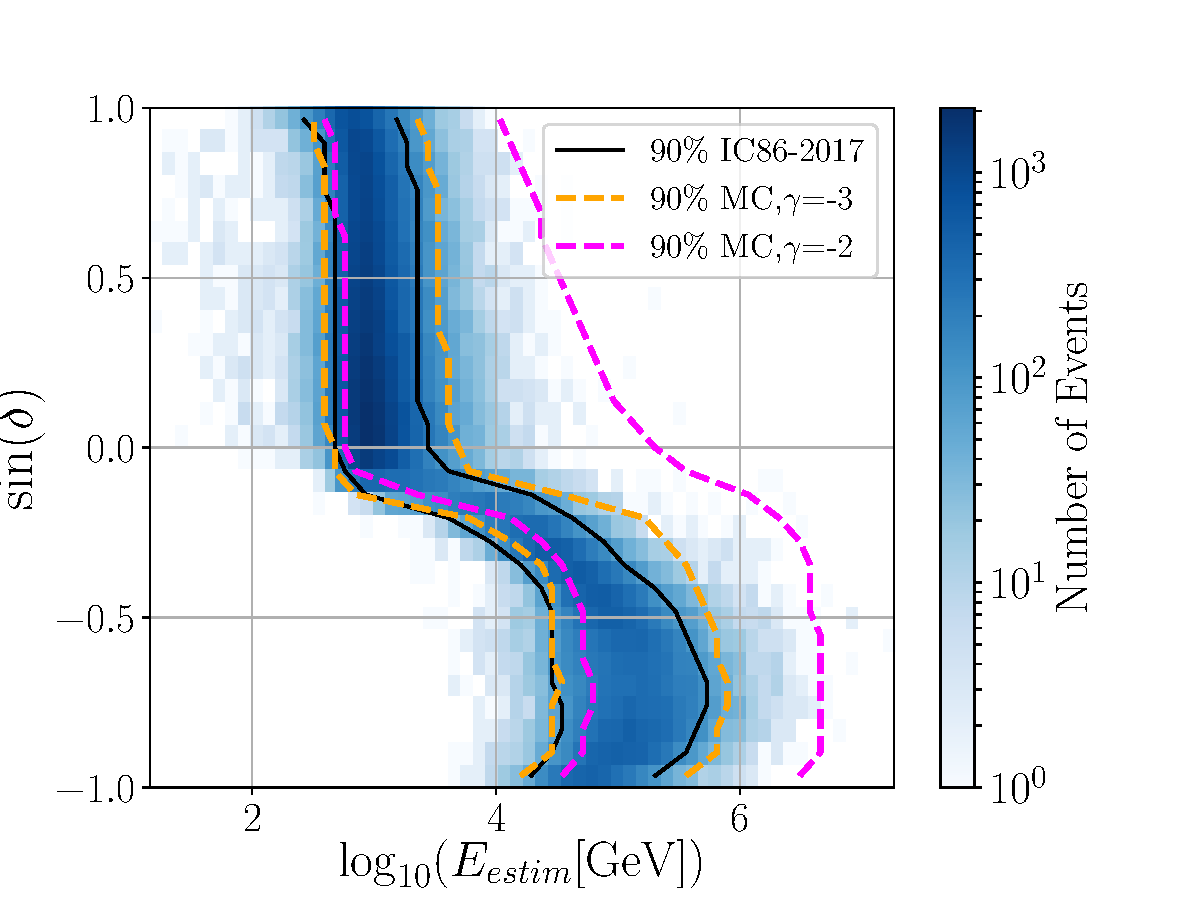
\includegraphics[width=\linewidth]{IC86II_enDist.pdf}
\caption[]{\MA{\it (To be updated.)} The distribution of events in one year of data for the final event selection as a function of reconstructed declination and estimated energy. The 90\% energy range for the data (black), as well as simulated astrophysical signal Monte-Carlo (MC) for an $E^{-2}$ and an $E^{-3}$ spectrum are shown in magenta and orange respectively as a guide for the relevant energy range of IceCube (from Ref.~\cite{Aartsen:2019fau}).}\label{fig:enDist}
\end{figure}
%%%%%%%%%%%%%%%%%

\section{Event Selection}

Different criteria are applied to select track-like events from the Northern and Southern hemisphere (with a boundary between them at declination $\delta=-5^\circ$), because the background differs in these two regions. Almost all the atmospheric muons in the Northern hemisphere can be removed by selecting high-quality track-like events. In the Southern hemisphere, the atmospheric background is reduced by strict cuts on the reconstruction quality and minimum energy, since the astrophysical neutrino fluxes are expected to have a harder energy spectrum than the background of atmospheric muons and neutrinos. This effectively removes almost all Southern hemisphere events with an estimated energy below $\simeq10$~TeV; see Fig.~\ref{fig:enDist}. 

In both hemispheres, atmospheric muons and cascade events are further filtered using multi-variate Boosted Decision Trees (BDT). In this analysis, a single BDT is trained to recognize three classes of events in the Northern hemisphere: single muon tracks from atmospheric and astrophysical neutrinos, atmospheric muons, and cascades, where neutrino-induced tracks are treated as signal. This BDT uses 11 variables related to event topology and reconstruction quality. The Northern BDT preserves $\sim90\%$ of the atmospheric neutrinos and $\sim0.1\%$ of the atmospheric muons from the initial selection of track-like events, also applied in previous muon neutrino searches~\cite{Aartsen:2016oji,Aartsen:2018ywr}. In the Southern hemisphere, the BDT and selection filters are taken from Ref.~\cite{Aartsen:2016oji}. The final all-sky event rate of $\sim2\,$mHz is dominated by muons from atmospheric neutrinos in the Northern hemisphere and by high-energy, well-reconstructed muons in the Southern hemisphere. This updated selection applied to the final 6 years of data shown in Table~\ref{tab:livetimes}. The preceding four years of data are handled exactly as in the past.

%%%%%%%%%%%%%%%%%
\begin{figure}[t]
\centering
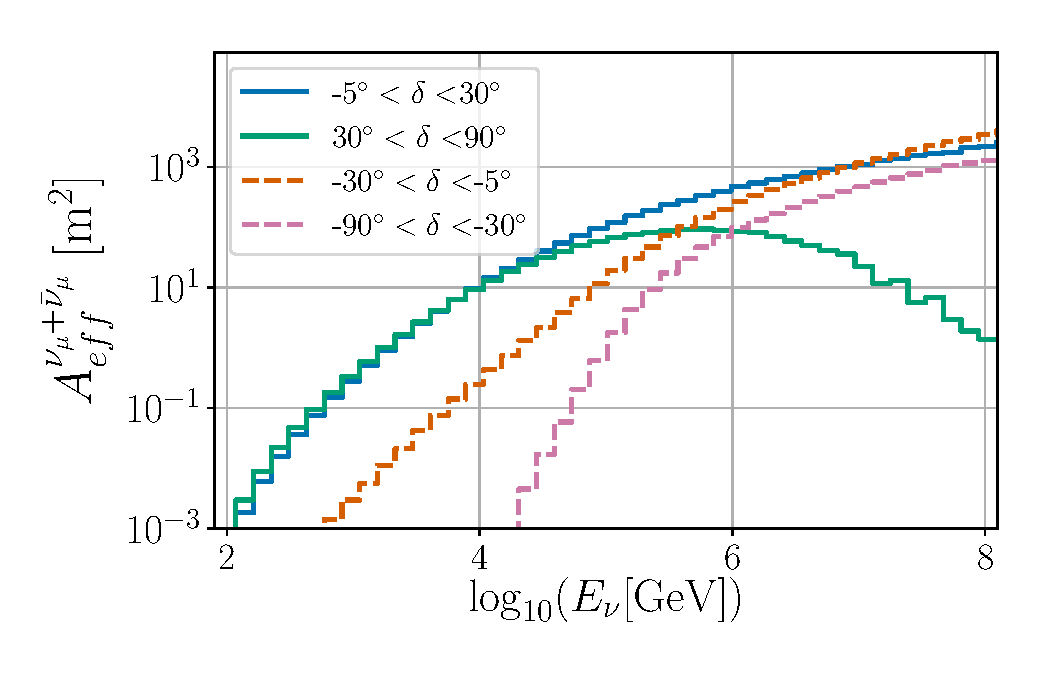
\includegraphics[width=\linewidth]{IC86II_effA.pdf}
\caption[]{\MA{\it (To be updated.)} The effective area as a function of neutrino energy for the IC86-II-VII event selection averaged across the declination band for several declination bins using simulated data (from Ref.~\cite{Aartsen:2019fau}).}\label{fig:effA}
\end{figure}
%%%%%%%%%%%%%%%%%

%%%%%%%%%%%%%%%%%
\begin{figure}[t]
\centering
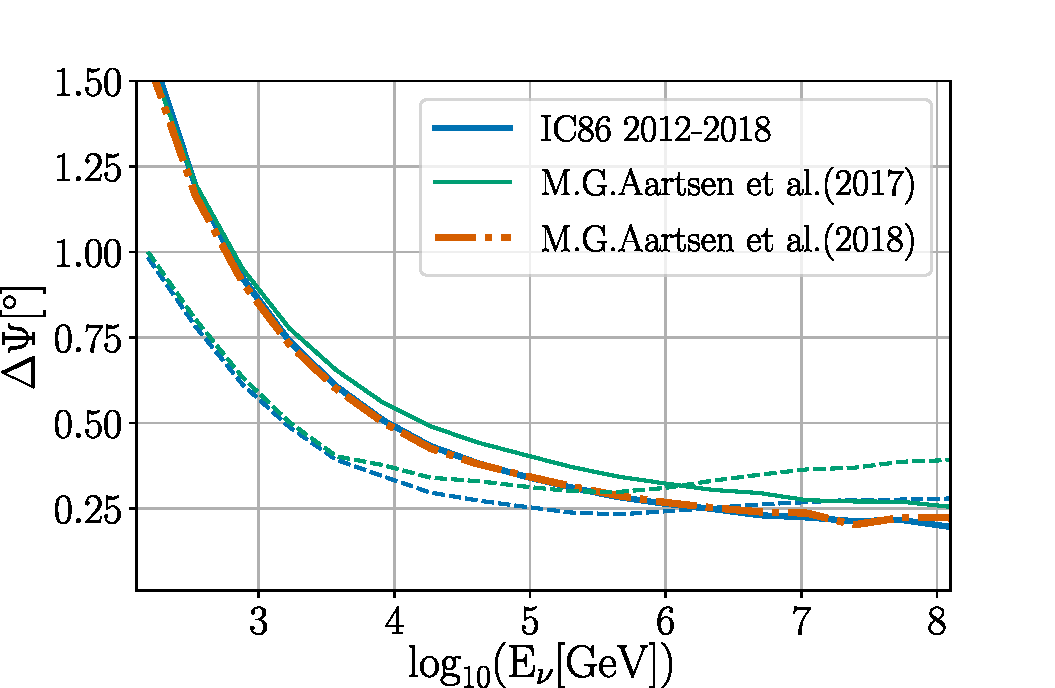
\includegraphics[width=\linewidth]{IC86II_PSF.pdf}
\caption[]{\MA{\it (To be updated.)} The median angle between simulated neutrino and reconstructed muon directions as a function of energy (from Ref.~\cite{Aartsen:2019fau}).}\label{fig:PSF}
\end{figure}
%%%%%%%%%%%%%%%%%

\section{Detector Response}

Muon tracks induced by astrophysical neutrino interactions are the main signal category in the search for point-like sources of neutrinos. Detailed Monte Carlo simulation is used to evaluate the response of IceCube to such events and distinguish them from atmospheric backgrounds. The median angular resolution $\Delta\Psi$ and the event rate expectation
\begin{align}\label{eq:ev_rate}
\dot{N}_\nu=\int d\Omega\int_0^\infty dE\,A_\mathrm{eff}\left(E, \Omega\right) \phi_\nu\left(E_\nu,\Omega\right)
\end{align}
given by the detector \emph{effective area} $A_\mathrm{eff}$ and the incident neutrino flux $\nu_\nu$ can be derived from the simulation; see \cite{Aartsen:2016xlq}.

\section{Comparison to Previous Releases}
There have been multiple previous IceCube data releases selecting for muon track-like events in the northern and southern hemisphere, primarily for the purpose of neutrino astronomy ~\cite{Abbasi:2010rd,Aartsen:2013uuv,IceCube:2018,IceCube:2019,IceCube:TXS2018}. The dataset detailed in this document is the newest such attempt at creating a sample of muon track-like events, with the goal of standardizing the IC86 2012-2017 data taking period. This dataset can be considered to be a successor to ~\cite{IceCube:2019}, providing an updated description of the data from 2012-2015, as well as adding two additional years of data in 2016-2017. 

While similar in goal and methods to ~\cite{IceCube:2019}, this sample includes several improvements in addition to the aforementioned standardization of the IC86 data taking periods. In this version of the data sample, the angular reconstruction has been improved, and the event classifier and sample pre-cuts have been altered to better reject cascade-like events and accept track-like events. The net effect of the sample changes is an increase in event rate relative to previous versions of the sample. In the IC86 2012-2015 data taking period, the new version of the data sample contains 362,818 events, in comparison to 338,588 in the previous version. Of these events, approximately 18\% (64,931 out of 362,818) are unique to the new version of the data sample, and are not present in older versions. Approximately 12\% (40,823 out of 338,588) of the events present in the older version of the sample are not present in the updated version presented here. 

As an example of how the changing content of the different versions of this data sample can affect the process of searching for hotspots in IceCube data, we examine the 2014/2015 neutrino flare associated with TXS 0506+056 ~\cite{IceCube:2018cha}. The $3.5 \sigma$ excess seen in in 2014/2015 was identified using the data sample corresponding to ~\cite{IceCube:2019}. Here, we repeat the analysis shown in ~\cite{IceCube:2018cha}, but instead use the newest data sample presented in this document. The results of this cross-check can be seen in table ~\ref{tab:TXSCrossChecks}. Notably, the significance of the 2014/2015 neutrino flare appears to have decreased (from $p=7.0 \times 10^{-5}$ to $p=8.1 \times 10^{-3}$) when using the most recent version of the data sample. A comparison of the reconstructed parameters of the most signal-like neutrino events contributing to the 2014/2015 flare in both versions of the data sample can be seen in table ~\ref{tab:TXSFlareEvtsTable}

The lower significance of the 2014/2015 neutrino flare in the most recent version of the sample appears to have been caused by the presence of two cascade-like events that existed in the data sample associated with ~\cite{IceCube:2019}, but have been removed from the data sample presented in this document. These two events did not pass a track length pre-cut that was introduced in the newest version of this data sample, requiring that all northern-sky events have a reconstructed track length greater than 200 meters. This pre-cut is intended to filter out poorly localized cascade events prior to applying the BDT. Performing the untriggered flare search using an older version of the sample (~\cite{IceCube:2019}), but with the two cascade events manually removed seems to result in a drop in significance similar to that which is observed when using this sample, as seen in table ~\ref{tab:TXSCrossChecks}. The drop in significance cannot be otherwise adequately explained by changes to the angular reconstruction of events between the two versions of the sample. Figure ~\ref{fig:TXSEvtsCompare} shows a comparison of the events most heavily contributing to the 2014/2015 TXS 0506+056 flare in both this data sample, and the most recent prior data release (~\cite{IceCube:2019}). While the significance of the 2014/2015 neutrino flare appears to have decreased when using the most recent version of the data sample, it should be noted that this is primarily a cross check between the new and old versions of the same data sample. The results are presented here primarily to demonstrate the differences between the old and new versions of this data sample. The results of this check do not supersede the results shown in ~\cite{IceCube:2018cha}.

\begin{figure*}[t]
\centering
\begin{minipage}{.5\textwidth}
  \centering
  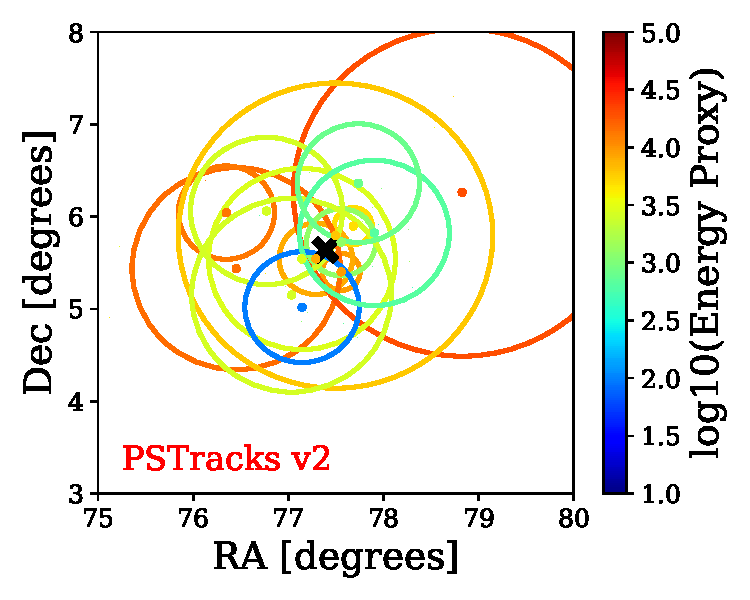
\includegraphics[width=.95\linewidth]{./TXSCheckPlots/PSTracksv2evtplot.pdf}
  \label{fig:test1}
\end{minipage}\hfill
\begin{minipage}{.5\textwidth}
  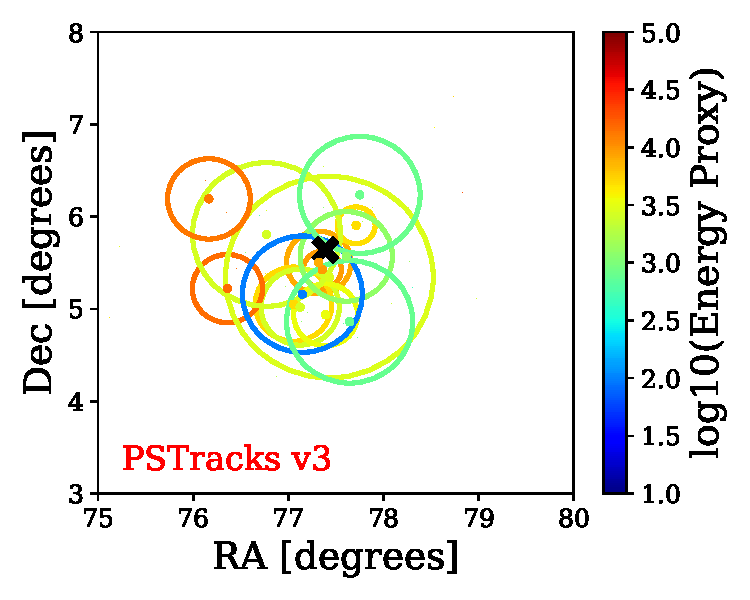
\includegraphics[width=.95\linewidth]{./TXSCheckPlots/PSTracksv3evtplot.pdf}
  \label{fig:test2}
\end{minipage}
\caption[]{The top 14 most signal-like flare events contributing to the 2014/2015 neutrino flare associated with TXS 0506+056 (black "X"), both in the sample associated with ~\cite{IceCube:2019} (left), and the sample presented in this document (right). The size of the colored circles corresponds to the 1-sigma containment region of the angular reconstruction of that event, and the color of the circle corresponds to the reconstructed energy proxy.}\label{fig:TXSEvtsCompare}
\end{figure*}

\begin{table*}
\centering
\begin{ruledtabular}
\begin{tabular}{cccccc}
\multicolumn{6}{c}{Cross-check Results} \\[0.1cm]
Sample & p-value (pre-trial) & $T_{start}$ & $T_{stop}$ & $n_s$ & $\gamma$\\ 
\cite{IceCube:2018cha}, \cite{IceCube:2019} & 7.0e-5 & 56937.81 & 57096.22 & 14.39 & 2.20 \\
This sample & 8.14e-3 & 56927.86 & 57116.76 & 11.87 & 2.22 \\
\cite{IceCube:2018cha}, removed cascades & 1.17e-3 & 56937.81 & 57112.65 & 12.22 & 2.26 \\
\end{tabular}
\end{ruledtabular}
\caption[]{The results of repeating the analysis done in ~\cite{IceCube:2018cha}, but using the dataset presented in this document in place of ~\cite{IceCube:2019}, the dataset that was originally used. The drop in significance when using this sample versus the older sample can be explained by events present in the older sample that have been removed from the newer sample presented here.}\label{tab:TXSCrossChecks}
\end{table*}

\begin{table*}
\centering
\begin{ruledtabular}
\begin{tabular}{c|cccc|cccc}
\multicolumn{1}{c|}{} &
\multicolumn{4}{c|}{2019 Data Release} & 
\multicolumn{4}{c}{2020 Data Release}\\[0.1cm]
Event ID & RA (deg) & Dec (deg) & $\sigma$ (deg) & $\log(E/GeV)$ & RA (deg) & Dec (deg) & $\sigma$ (deg) & $\log(E/GeV)$\\ 
\hline
63641159 & 77.55 & 5.40 & 0.20 & 3.97 & 77.35 & 5.42 & 0.20 & 3.97\\
5363166 & 77.28 & 5.54 & 0.38 & 3.91 & 77.32 & 5.50 & 0.34 & 3.91\\
55370999 & 77.68 & 5.89 & 0.20 & 3.69 & 77.71 & 5.90 & 0.20 & 3.69\\
52497651 & 76.45 & 5.43 & 1.09 & 4.17 & 76.35 & 5.22 & 0.36 & 4.71\\
56262988 & 78.82 & 6.26 & 1.77 & 4.30 & - & - & - & - \\
502182 & 76.34 & 6.04 & 0.50 & 4.13 & 76.16 & 6.19 & 0.43 & 4.13 \\
44740885 & 77.55 & 5.72 & 0.36 & 3.09 & 77.60 & 5.56 & 0.48 & 3.0 \\
40914587 & 77.49 & 5.79 & 1.65 & 3.79 & - & - & - & -  \\
26587403 & 77.14 & 5.54 & 0.98 & 3.46 & 77.43 & 5.34 & 1.09 & 3.46 \\
769297 & 76.77 & 6.06 & 0.79 & 3.42 & 76.77 & 5.80 & 0.77 & 3.42 \\
24269091 & 77.03 & 5.14 & 1.05 & 3.43 & 76.35 & 5.22 & 0.36 & 4.17 \\
30121650 & 77.14 & 5.01 & 0.60 & 1.99 & 77.14 & 5.15 & 0.63 & 1.99 \\
51031373 & 77.90 & 5.82 & 0.78 & 2.82 & - & - & - & - \\
63708451 & 77.73 & 6.36 & 0.64 & 2.91 & 77.75 & 6.23 & 0.63 & 2.91 \\
54221887 & - & - & - & - & 77.05 & 5.05 & 0.40 & 3.71 \\
1939266 & - & - & - & - & 77.39 & 4.93 & 0.33 & 3.53 \\
\end{tabular}
\end{ruledtabular}
\caption[]{The most signal-like events contributing to the 2014/2015 TXS 0506+056 neutrino flare, in both the data sample associated with ~\cite{IceCube:2019}, as well as the data sample presented here. There were no changes to energy reconstruction between the two sample versions, but the angular reconstruction and sample event content have changed.}\label{tab:TXSFlareEvtsTable}
\end{table*}

\begin{acknowledgements}
\begin{center}\MA{(\it List of agencies in final version)}\end{center}
%USA {\textendash} U.S. National Science Foundation-Office of Polar Programs,
U.S. National Science Foundation-Physics Division,
Wisconsin Alumni Research Foundation,
Center for High Throughput Computing (CHTC) at the University of Wisconsin{\textendash}Madison,
Open Science Grid (OSG),
Extreme Science and Engineering Discovery Environment (XSEDE),
U.S. Department of Energy-National Energy Research Scientific Computing Center,
Particle astrophysics research computing center at the University of Maryland,
Institute for Cyber-Enabled Research at Michigan State University,
and Astroparticle physics computational facility at Marquette University;
Belgium {\textendash} Funds for Scientific Research (FRS-FNRS and FWO),
FWO Odysseus and Big Science programmes,
and Belgian Federal Science Policy Office (Belspo);
Germany {\textendash} Bundesministerium f{\"u}r Bildung und Forschung (BMBF),
Deutsche Forschungsgemeinschaft (DFG),
Helmholtz Alliance for Astroparticle Physics (HAP),
Initiative and Networking Fund of the Helmholtz Association,
Deutsches Elektronen Synchrotron (DESY),
and High Performance Computing cluster of the RWTH Aachen;
Sweden {\textendash} Swedish Research Council,
Swedish Polar Research Secretariat,
Swedish National Infrastructure for Computing (SNIC),
and Knut and Alice Wallenberg Foundation;
Australia {\textendash} Australian Research Council;
Canada {\textendash} Natural Sciences and Engineering Research Council of Canada,
Calcul Qu{\'e}bec, Compute Ontario, Canada Foundation for Innovation, WestGrid, and Compute Canada;
Denmark {\textendash} Villum Fonden, Danish National Research Foundation (DNRF), Carlsberg Foundation;
New Zealand {\textendash} Marsden Fund;
Japan {\textendash} Japan Society for Promotion of Science (JSPS)
and Institute for Global Prominent Research (IGPR) of Chiba University;
Korea {\textendash} National Research Foundation of Korea (NRF);
Switzerland {\textendash} Swiss National Science Foundation (SNSF);
United Kingdom {\textendash} Department of Physics, University of Oxford.
\end{acknowledgements}

\bibliographystyle{utphys_mod}

\bibliography{references}

\end{document}

